\documentclass[12pt,prb,aps,notitlepage]{revtex4-1}
\usepackage {amsmath}
\usepackage{amssymb}
\pdfoutput = 1 
\usepackage {graphicx}
\newcommand{\bomega}{\mbox{\boldmath$\omega$}}
\newcommand{\bxi}{\mbox{\boldmath$\xi$}}
\newcommand{\bbeta}{\mbox{\boldmath$\beta$}}
\allowdisplaybreaks

\begin{document}

\title{Benchmark of TJ Code Against STRIDE Code}
\author{R.~Fitzpatrick\,\footnote{rfitzp@utexas.edu}}
\affiliation{Institute for Fusion Studies,  Department of Physics,  University of Texas at Austin,  Austin TX 78712, USA}\begin{abstract}
\end{abstract}
\maketitle

\section{Symmetry Relations}
Let  all lengths be normalized to the major radius of the magnetic axis, $R_0$,  and let
all magnetic field-strengths be normalized to  the toroidal magnetic field-strength at the axis, $B_0$. 
Consider an axisymmetric toroidal plasma equilibrium. 
Let $R$, $\phi$, $Z$ be a conventional cylindrical coordinate system that is co-axial
with the toroidal symmetry axis of the plasma. 
The equilibrium magnetic field is written
\begin{equation}
{\bf B} =\nabla\phi\times \nabla\psi+g(\psi)\,\nabla\psi,
\end{equation}
where $\psi$ is the  poloidal magnetic flux. We can also
define 
\begin{equation}
{\mit\Psi}_N = \frac{\psi}{\psi_a},
\end{equation}
where $\psi_a$ is the poloidal flux at the plasma boundary. Thus, ${\mit\Psi}_N=0$ at the magnetic axis, and
${\mit\Psi}_N=1$ on the plasma boundary. In the following, it is assumed that ${\mit\Psi}_N$ is the `radial'
coordinate in STRIDE. 

Let
\begin{align}
L_m^m({\mit\Psi}_N) &= I({\mit\Psi}_N)\left( J({\mit\Psi}_N)\left[\frac{m\,g({\mit\Psi}_N)}{q({\mit\Psi}_N)}\right]^2+ [n\,\psi_a]^2\right),\\[0.5ex]
I({\mit\Psi}_N) &= \int_0^{{\mit\Psi}_N} \frac{2\,q\,({\mit\Psi}_N')}{g({\mit\Psi}_N')}\,d{\mit\Psi}_N',\\[0.5ex]
J({\mit\Psi}_N)&= \oint|\nabla{\mit\Psi}_N|^{-2}\,\frac{d\theta}{2\pi},\\[0.5ex]
\rho({\mit\Psi}_N) &= \frac{J({\mit\Psi}_N)\,g({\mit\Psi}_N)}{q({\mit\Psi}_N)},\\[0.5ex]
s({\mit\Psi}_N) &= \frac{d\ln q}{d{\mit\Psi}_N},
\end{align}
where $m$ is a poloidal mode number, $n$ is a toroidal mode number, $q({\mit\Psi}_N)$ is the safety-factor, and $\theta$ is
a `straight' poloidal  angle defined such that 
\begin{equation}
(\nabla\phi\times\nabla\theta\cdot\nabla\phi)^{-1} = \frac{q\,R^2}{g},
\end{equation}
Note that we are working in PEST coordinates. 

Let $m_j$ be the poloidal mode number of the $j$th rational surface, which is located at ${\mit\Psi}_N= {\mit\Psi}_{N\,j}$. Let $D_{I\,j}$ be the ideal
Mercier index at the $j$th rational surface, and
let
\begin{align}
\nu_{L\,j} &=\frac{1}{2}-\sqrt{-D_{I\,j}},\\[0.5ex]
\nu_{S\,j} &=\frac{1}{2}+\sqrt{-D_{I\,j}}.
\end{align}
Let
\begin{align}
f_{L\,j} &= \left[\rho^{\,\nu_{L\,j}}
\left(\frac{\nu_{S\,j}-\nu_{L\,j}}{L_{m_j}^{m_j}}\right)^{1/2}\,s\,m_j
\right]_{{\mit\Psi}_{N\,j}},\\[0.5ex]
f_{S\,j} &= \left[\rho^{\,\nu_{S\,j}}
\left(\frac{\nu_{S\,j}-\nu_{L\,j}}{L_{m_j}^{m_j}}\right)^{1/2}\,s\,m_j
\right]_{{\mit\Psi}_{N\,j}}.
\end{align}
Finally, let
\begin{align}
\hat{A}_{ij}&= f_{S\,j}^{\,-1}\,A_{ij}\,f_{L\,j'},\\[0.5ex]
\hat{B}_{ij}&= f_{S\,j}^{\,-1}\,B_{ij}\,f_{L\,j'},\\[0.5ex]
\hat{\mit\Gamma}_{ij}&= f_{S\,j}^{\,-1}\,{\mit\Gamma}_{ij}\,f_{L\,j'},\\[0.5ex]
\hat{\mit\Delta}_{ij}&= f_{S\,j}^{\,-1}\,{\mit\Delta}_{ij}\,f_{L\,j'},
\end{align}
where $A_{ij}$, $B_{ij}$, ${\mit\Gamma}_{ij}$, and ${\mit\Delta}_{ij}$ are the elements of the outer matching matrices
calculated by STRIDE, whereas the hatted quantities are the  corresponding matching matrices calculated by TJ. 
Equations~(77) and (100) of Ref.~\onlinecite{pletzer} imply that
\begin{align}
\hat{A}_{ji}^\ast &= \hat{A}_{ij},\\[0.5ex]
\hat{\mit\Delta}_{ji}^\ast &= \hat{\mit\Delta}_{ij},\\[0.5ex]
\hat{B}_{ji}^\ast &= \hat{\mit\Gamma}_{ij}.
\end{align}
These symmetries are ultimately due to the self-adjoint nature of the ideal-MHD force operator. However, as explained
in Ref.~\onlinecite{rf}, the symmetries can also be related to the conservation of toroidal electromagnetic angular momentum. The
symmetries have to be respected by a toroidal tearing mode code, otherwise the code would predict that an isolated 
plasma could exert a net toroidal electromagnetic torque on itself. Note that, in the cylindrical limit, $\hat{\mit\Delta}_{jj}$ is equivalent to $r_s\,{\mit\Delta}'$: i.e.,
the tearing stability index normalized to the minor radius of the rational surface. 

\section{TJ/STRIDE/TEAR  Equilibrium}
The TJ/STRIDE/TEAR large-aspect ratio, circular,  plasma equilibrium  has a Wesson-like current profile\,\cite{wesson} characterized by the
safety-factor on the magnetic axis, $q_0$, and the safety-factor at the plasma boundary, $q_a$. 
The
 parallel current profile, $\sigma={\bf J}\cdot{\bf B}/B^2$,  is written
\begin{equation}
\sigma(r) = \frac{2}{q_0}\left[1-\left(\frac{r}{a}\right)^2\right]^{p_\sigma}.
\end{equation}
whereas the a  pressure profile takes the form
\begin{equation}
p(r)= \frac{\beta_0}{2}\left[1-\left(\frac{r}{a}\right)^2\right]^{p_p}.
\end{equation}
Here, $r$ is the flux surface label defined in Ref.~\onlinecite{rf}. Moreover, the magnetic axis corresponds to $r=0$, and the plasma
boundary to $r=a$. A STRIDE equilibrium is defined by the parameters $q_0$, $p_\sigma$, $\beta_0$, and $p_p$. In TJ equilibria,
$q_0$, $\beta_0$, and $p_p$ are the same as in STRIDE, but $p_\sigma$ is adjusted to obtain the same $q_a$ value as in STRIDE. 
TEAR equilibria are specified by $q_0$ and $q_a$. 
The TJ and STRIDE equilibria are also characterized by the inverse aspect-ratio of the plasma, $\epsilon_a$. The TEAR equilibria are such that
$\epsilon_a=0$. 

\section{Benchmark Tests}
\subsection{Single Rational Surface}
We consider the stability of $n=1$ tearing modes 
in a zero pressure equilibrium that only contain a single $n=1$ rational surface: namely, the 2/1 surface. 

\subsubsection{Test 1}
The first test has equilibria characterized by $q_0=1.1$ and $p_\sigma=1.36$ (in STRIDE), with a range of different inverse aspect-ratios, $\epsilon_a$. 
Figure~1 compares the $\hat{\mit\Delta}_{11}$ (i.e.,
the tearing stability index of the 2/1 tearing mode) values calculated by the TJ code,\cite{tj} the TEAR code (which is a cylindrical tearing mode code), and
the STRIDE code. It can be seen that the tearing stability indices calculated by the TJ and STRIDE are in good agreement, and asymptote to that calculated by the TEAR code
in the cylindrical limit, $\epsilon_a\rightarrow 0$. 

\subsubsection{Test 2}
The second test has equilibria characterized by $q_0=1.1$ and $\epsilon_a=0.2$, with a range of edge safety-factor values, $q_a$. 
Figure~2 compares the $\hat{\mit\Delta}_{11}$ (i.e.,
the tearing stability index of the 2/1 tearing mode) values calculated by the TJ code, the TEAR code, and
the STRIDE code. It can be seen that the tearing stability indices calculated by the TJ and STRIDE are in good agreement, except when the $q=3$ surface closely approaches the
plasma boundary (i.e., $q_a\rightarrow 3$). 
 
 \subsection{Two Rational Surfaces}
 We consider the stability of $n=1$ tearing modes 
in a zero pressure equilibrium  that  contains two $n=1$ rational surface: namely, the 2/1 surface and the 3/1 surface. 

\subsubsection{Test 3}
The third test has equilibria characterized by $q_0=1.1$ and $\epsilon_a=0.2$, with a range of edge safety-factor values, $q_a$. 
Figure~3 compares the elements of the tearing stability matrix calculated by the TJ and the STRIDE codes. It can be seen that the elements calculated by
TJ and STRIDE are in good agreement. 

\section*{References}
\begin{thebibliography}{99}\baselineskip 5ex

\bibitem{pletzer} A.~Pletzer, A.~Bondeson, and R.L.~Dewar, J.\ Comp.\ Phys.\ {\bf 115}, 530 (1994).

\bibitem{rf} R.~Fitzpatrick, Phys.\ Plasmas {\bf 1}, 3308 (1994). 

\bibitem{wesson} J.A.~Wesson, Nucl.\ Fusion {\bf 18},  87 (1978). 

\bibitem{tj} R.~Fitzpatrick, Phys.\ Plasmas {\bf 31}, 102507 (2024).

\end{thebibliography}

\newpage
\begin{figure}
\centerline{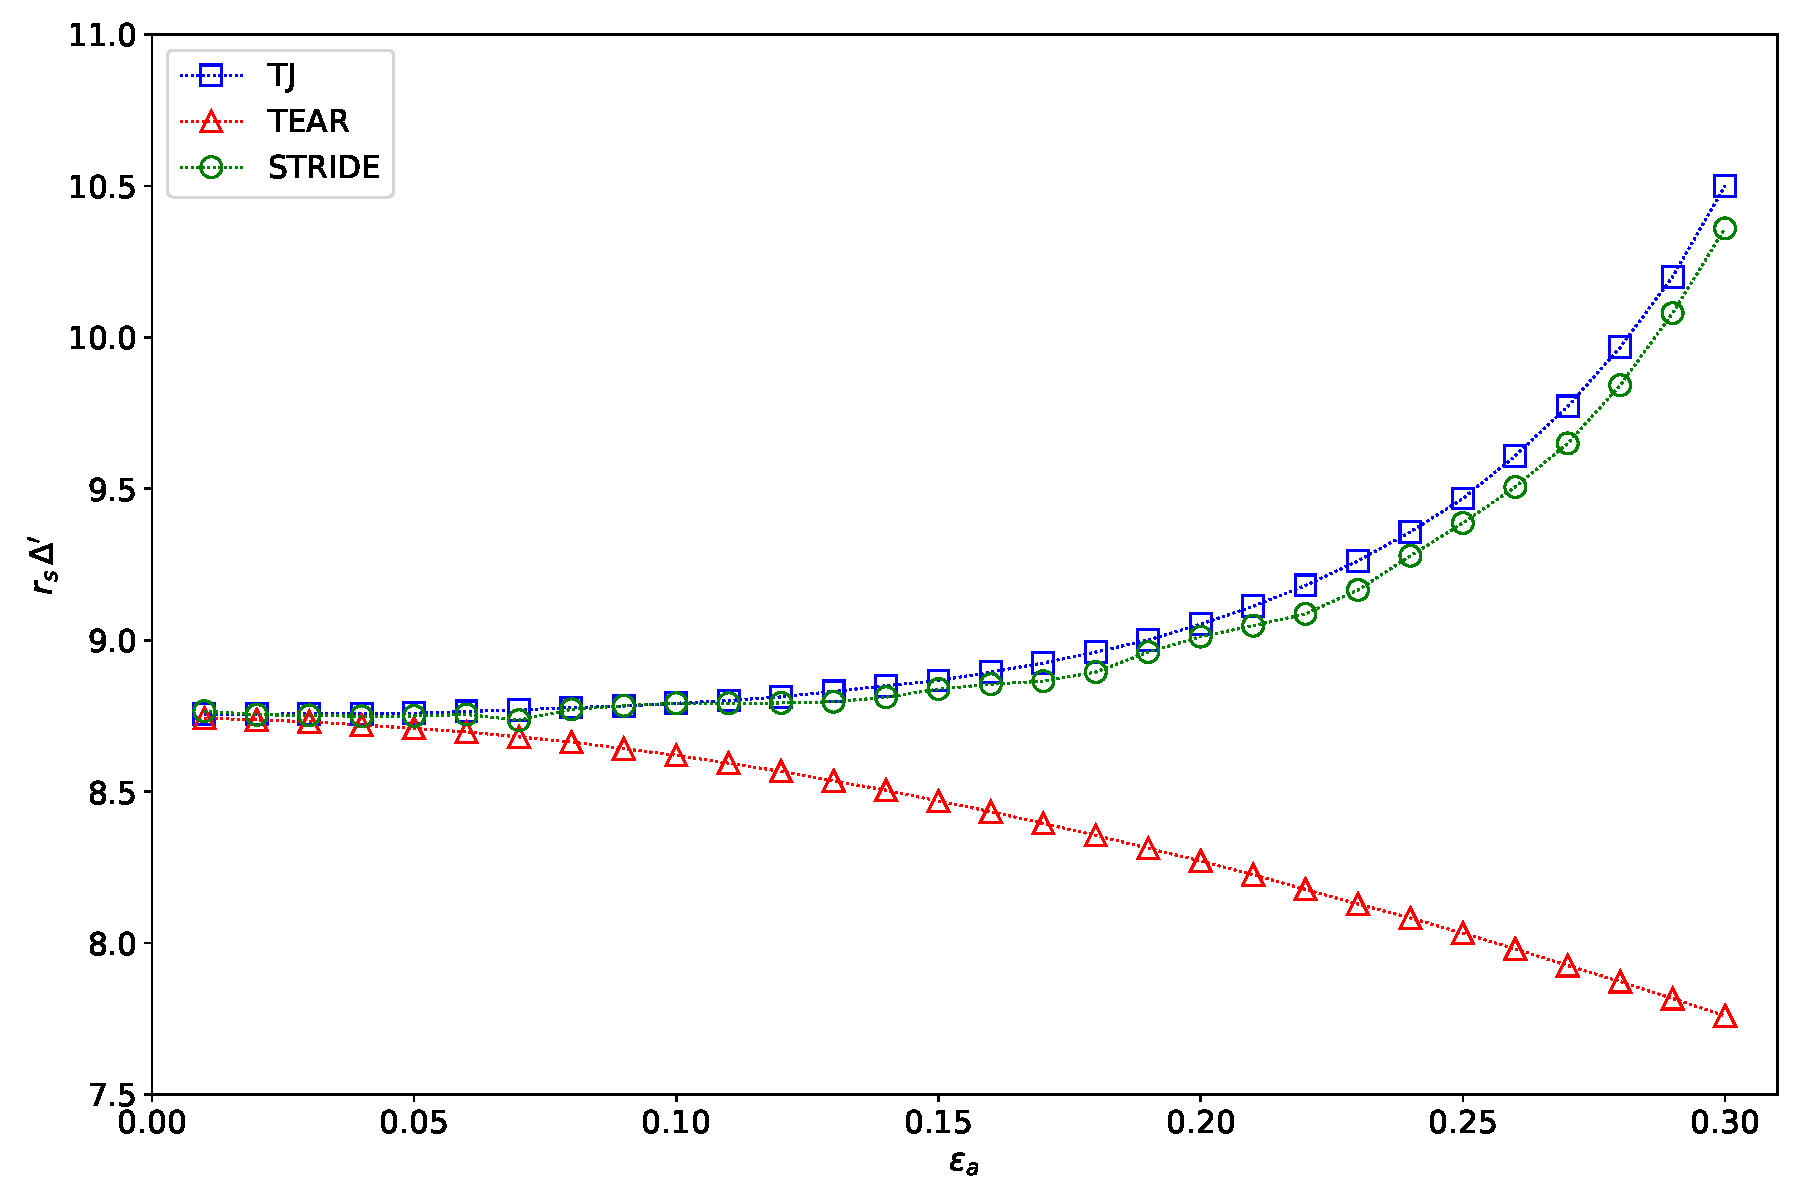
\includegraphics[width=\textwidth]{Test1.pdf}}
\caption{Test 1: $q_0=1.1$, $p_\sigma=1.36$ (STRIDE), $\beta_0=0.0$. Variation of 2/1 tearing stability index with inverse-aspect ratio, $\epsilon_a$. }
\end{figure}

\newpage
\begin{figure}
\centerline{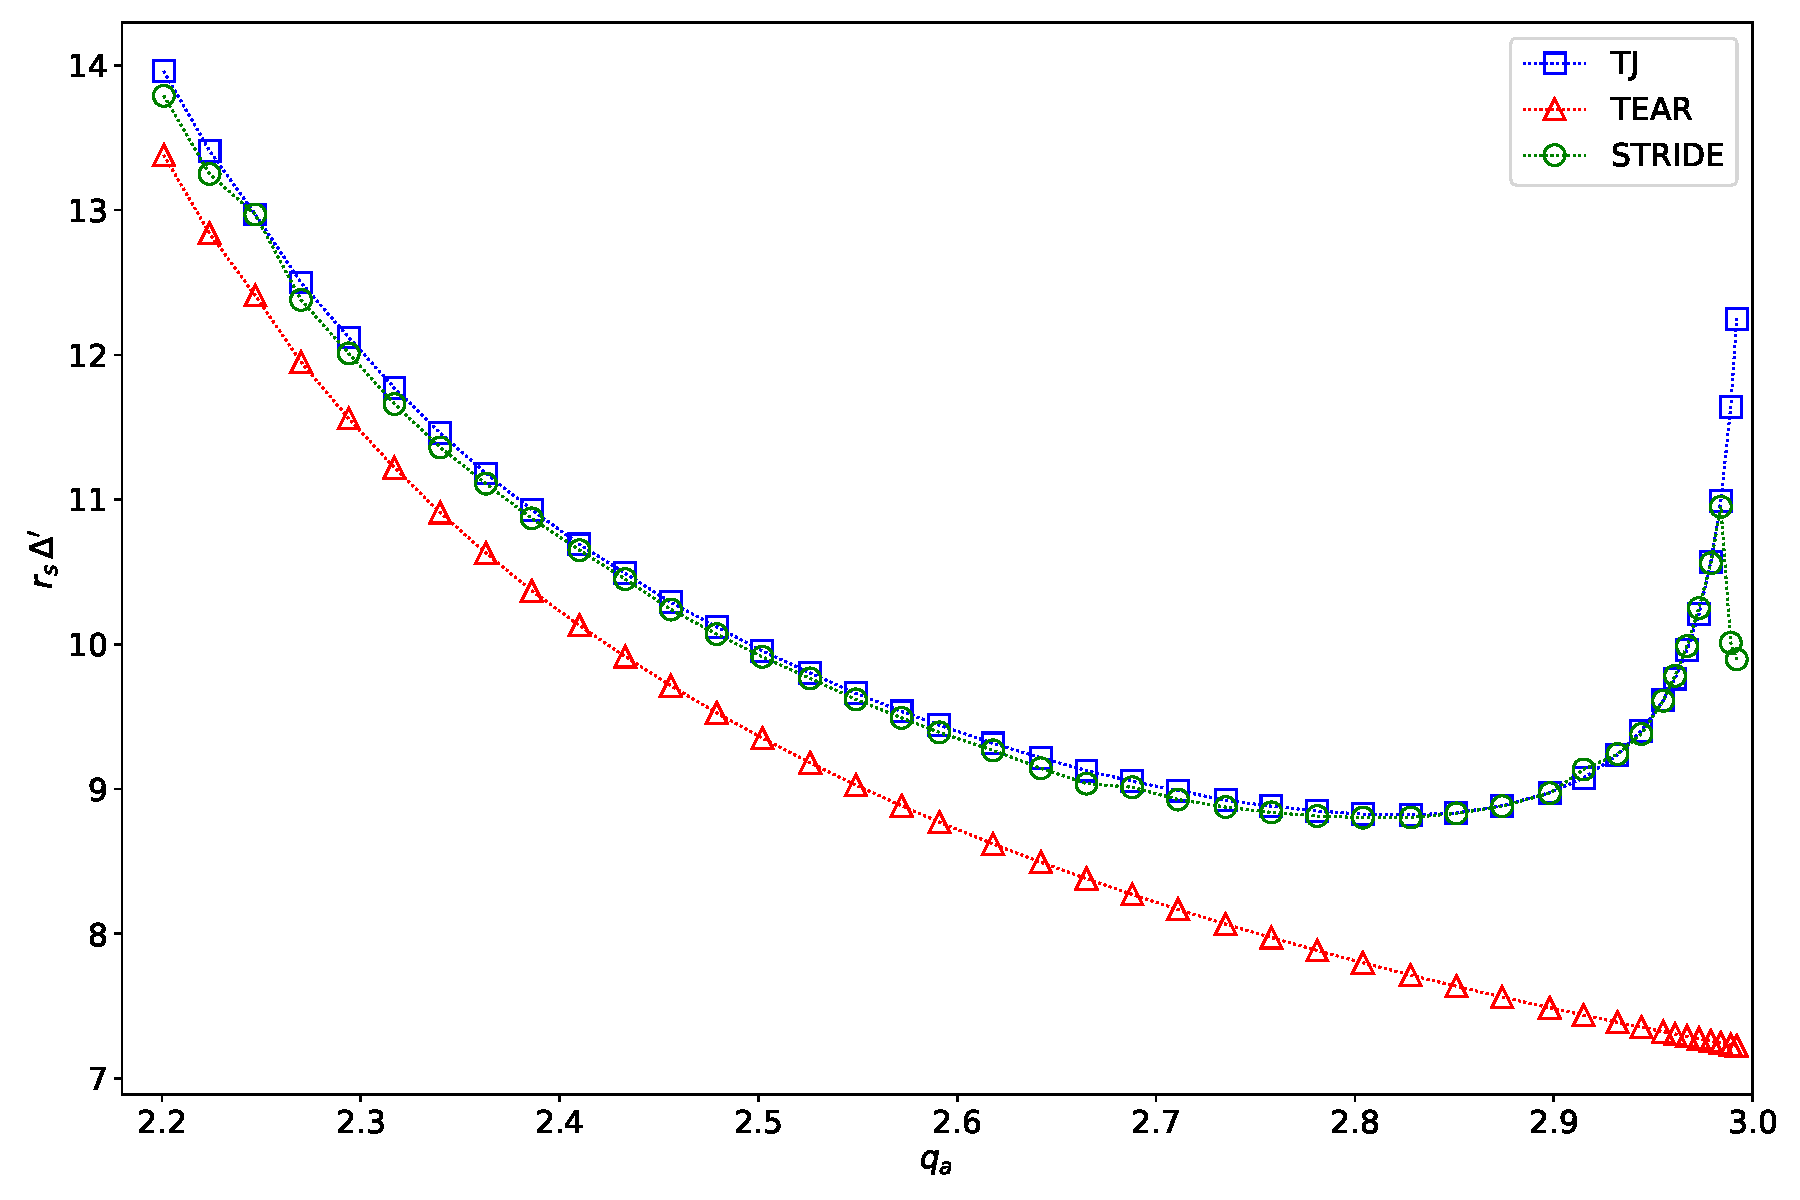
\includegraphics[width=\textwidth]{Test2.pdf}}
\caption{Test 2: $q_0=1.1$, $\epsilon_a=0.2$, $\beta_0=0.0$. Variation of 2/1 tearing stability index with $q_a$. }
\end{figure}

\newpage
\begin{figure}
\centerline{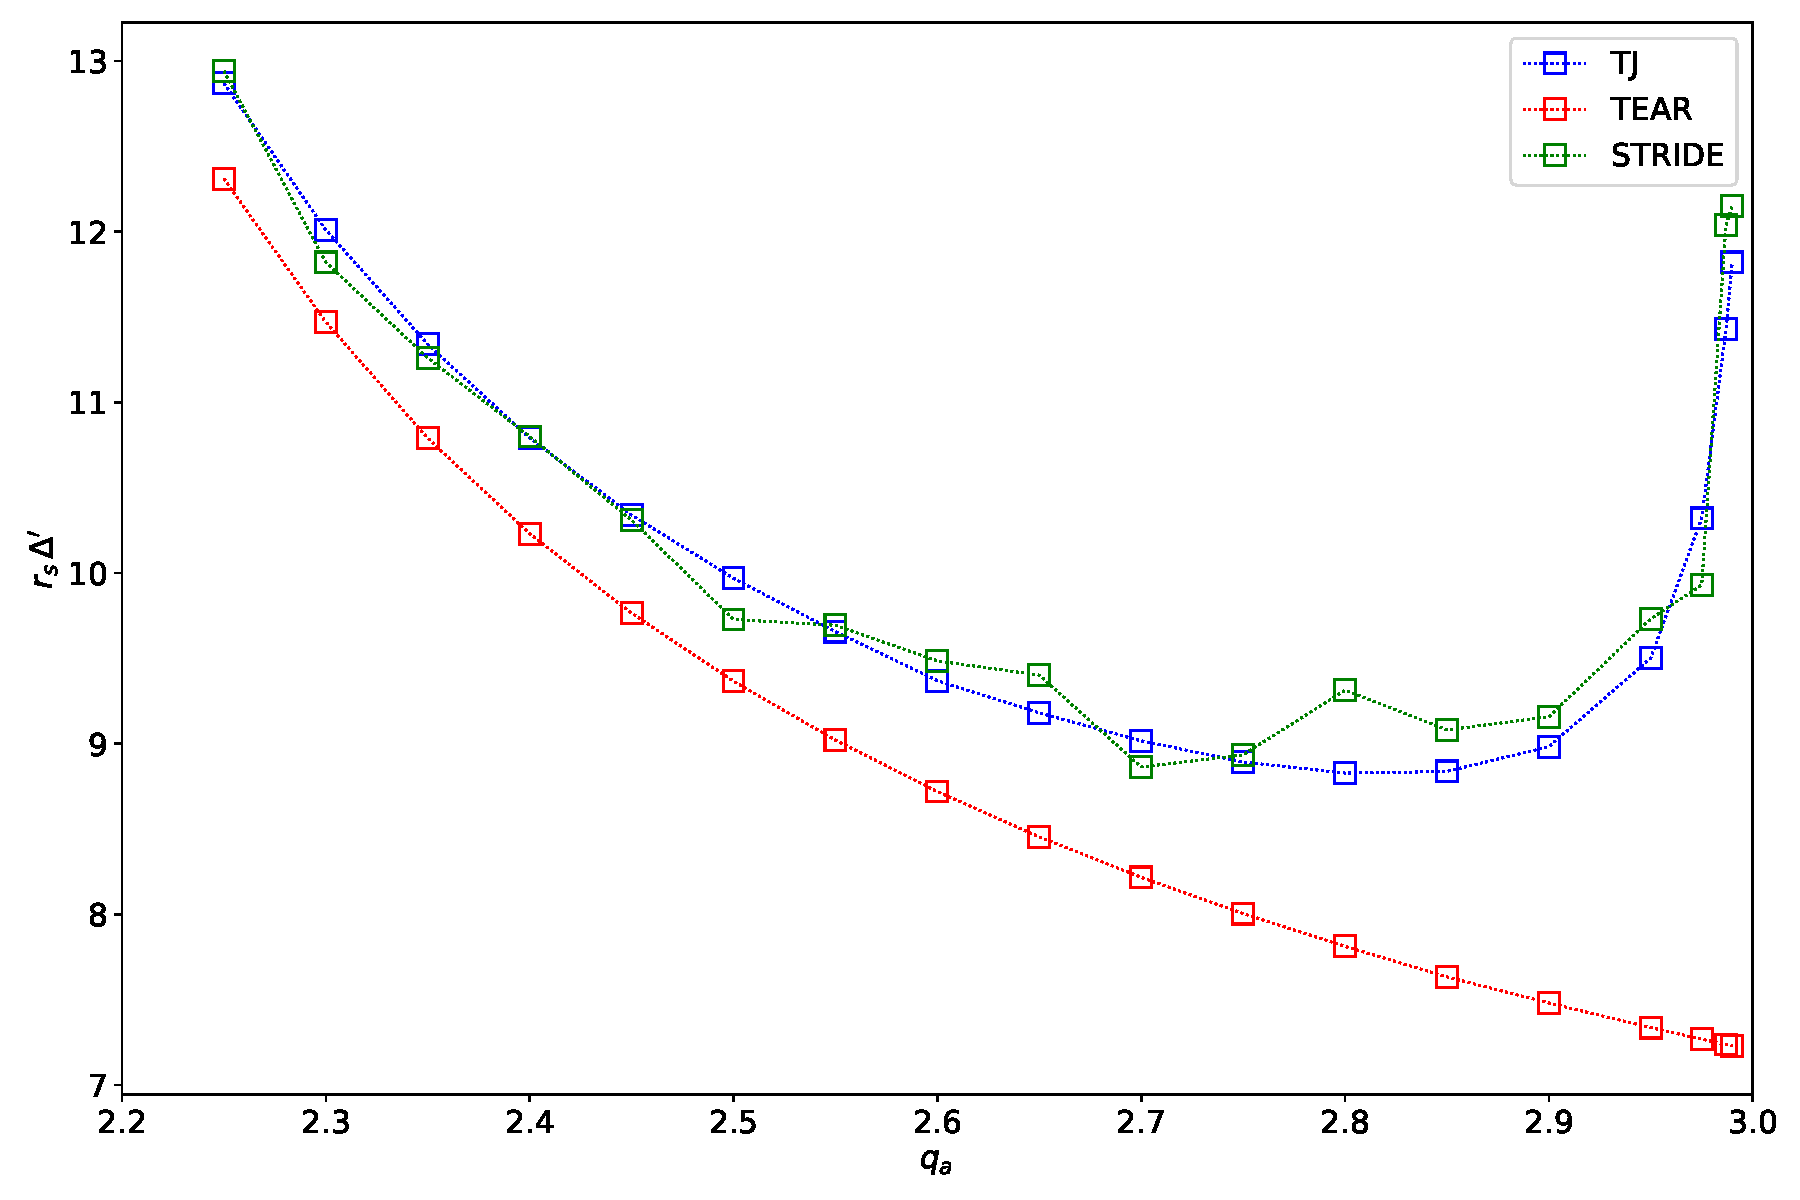
\includegraphics[width=\textwidth]{Test3.pdf}}
\caption{Test 3: $q_0=1.1$, $\epsilon_a=0.2$, $\beta_0=0.0$. Variation of elements of tearing stability matrix with $q_a$. In the middle panels the squares
indicate  $E_{12}$ and the crosses indicate $E_{21}$. }
\end{figure}





\end{document}

